
\documentclass{article}
\usepackage{times}
\usepackage{graphicx} 
\usepackage{subfigure}
\usepackage{natbib}
\usepackage{algorithm}
\usepackage{algorithmic}
\usepackage{hyperref}
\newcommand{\theHalgorithm}{\arabic{algorithm}}
\usepackage[accepted]{icml2015}

\icmltitlerunning{}

\begin{document} 

\twocolumn[
	\icmltitle{CMPS 242 - Machine Learning (Final Report) \\ Analysis of Rating Dimensions Using Review Text}

	\icmlauthor{Bharath Nagesh}{\textit{bnagesh@ucsc.edu}}
	\icmlauthor{Madhu Shivashankaraiah}{\textit{mshivash@ucsc.edu}}
	\icmlauthor{Numra Bathool}{\textit{nbathool@ucsc.edu}}
	\icmlauthor{Tanay Parekhji}{\textit{tparekhji@ucsc.edu}}

	\vskip 0.1in

	\icmlauthor{Git repository link : }{\textit{\textbf{\texttt{https://github.com/madhusedu/topic\_modeling.git}}}}
	\icmlkeywords{CMPS 242 Project Report}

	\vskip 0.3in
]

\begin{abstract} 


	Modern day systems take in both ratings and review texts from the user but generally consider only the ratings for 	
	performing different tasks, such as predictions and assessing the overall quality of a business. This according to us is not 
	the optimal method. Ratings are highly subjective and what might be considered as favorable by one could be unfavorable 
	for another. After a detailed observation of the review texts on IMDb, Zomato and Yelp we noticed that users implicitly 
	provide information on their likes and dislikes. We plan to implement a system which takes in not only the rating but also 
	the review text in order to form an opinion. We consider all the reviews of the users and then use data mining to 
	summarize them. We also classify some reviews belonging to the same topic.  form an opinion on the preferences of the 
	users, then finally use those opinions in order to improve the overall rating quality for the business and perform better user 
	predictions.

\end{abstract} 

\section{Problem Statement}
	\label{problem}

		Along with the expansion of the internet, a number of services such as e-Commerce and Review websites have 	
		emerged. A lot of people prefer using these services because of many factors, some of them being :

	\begin{itemize}
		\item{\textbf{Reliability :} These services provide excellent delivery of product/information and then back it up with a 
		good level of customer care. Also, the ratings provided on these sites aren't just a number that is just floated 
		to hoodwink the customer into buying the product/using the service making them very reliable}
		\item{\textbf{Ease of use :} All these services have a clean web/app interface which makes it very convenient for the 
		people to use them. }
\end{itemize}
The effect of the above factors can be seen in the growth of the industries, as indicated in Figure. ~\ref{sales} and Figure ~\ref{yelp}.

During holidays such as Thanksgiving the use of these services increase dramatically. The usage statistics is indicated in Figure ~\ref{thanksgiving}.

The general method used to increase the reliability of a product/business/service is by collecting ratings reviews from the people who have used them. This facilitates future customers to form a better opinion of the product when deciding to whether or not use the product.  

After a thorough observation of ratings and reviews provided on websites such as IMDb, Yelp, Amazon the following was observed. The overall rating for any product is formed as a weighted average of the ratings provided by all the users. This method completely disregards the review text provided by many of the users.  The users generally provide important information which can be used to improve the overall rating of the product. For an example of this situation, we can consider reviews provided for a restaurant. An user may provide a rating of 3 stars for the restaurant and then provide a review which makes the restaurant actually worth 3.5 or maybe even 4 stars. 

This problem that is presented above provided us with the opportunity to develop a system which uses Latent Dirichlet Allocation and Topic Modeling techniques in order to understand the reviews provided by the user. After doing so we attempt to develop an application which fine tunes the overall quality of ratings for any given product/business. 


\begin{figure}[ht]
	\vskip 0.2in
		\begin{center}
			\centerline{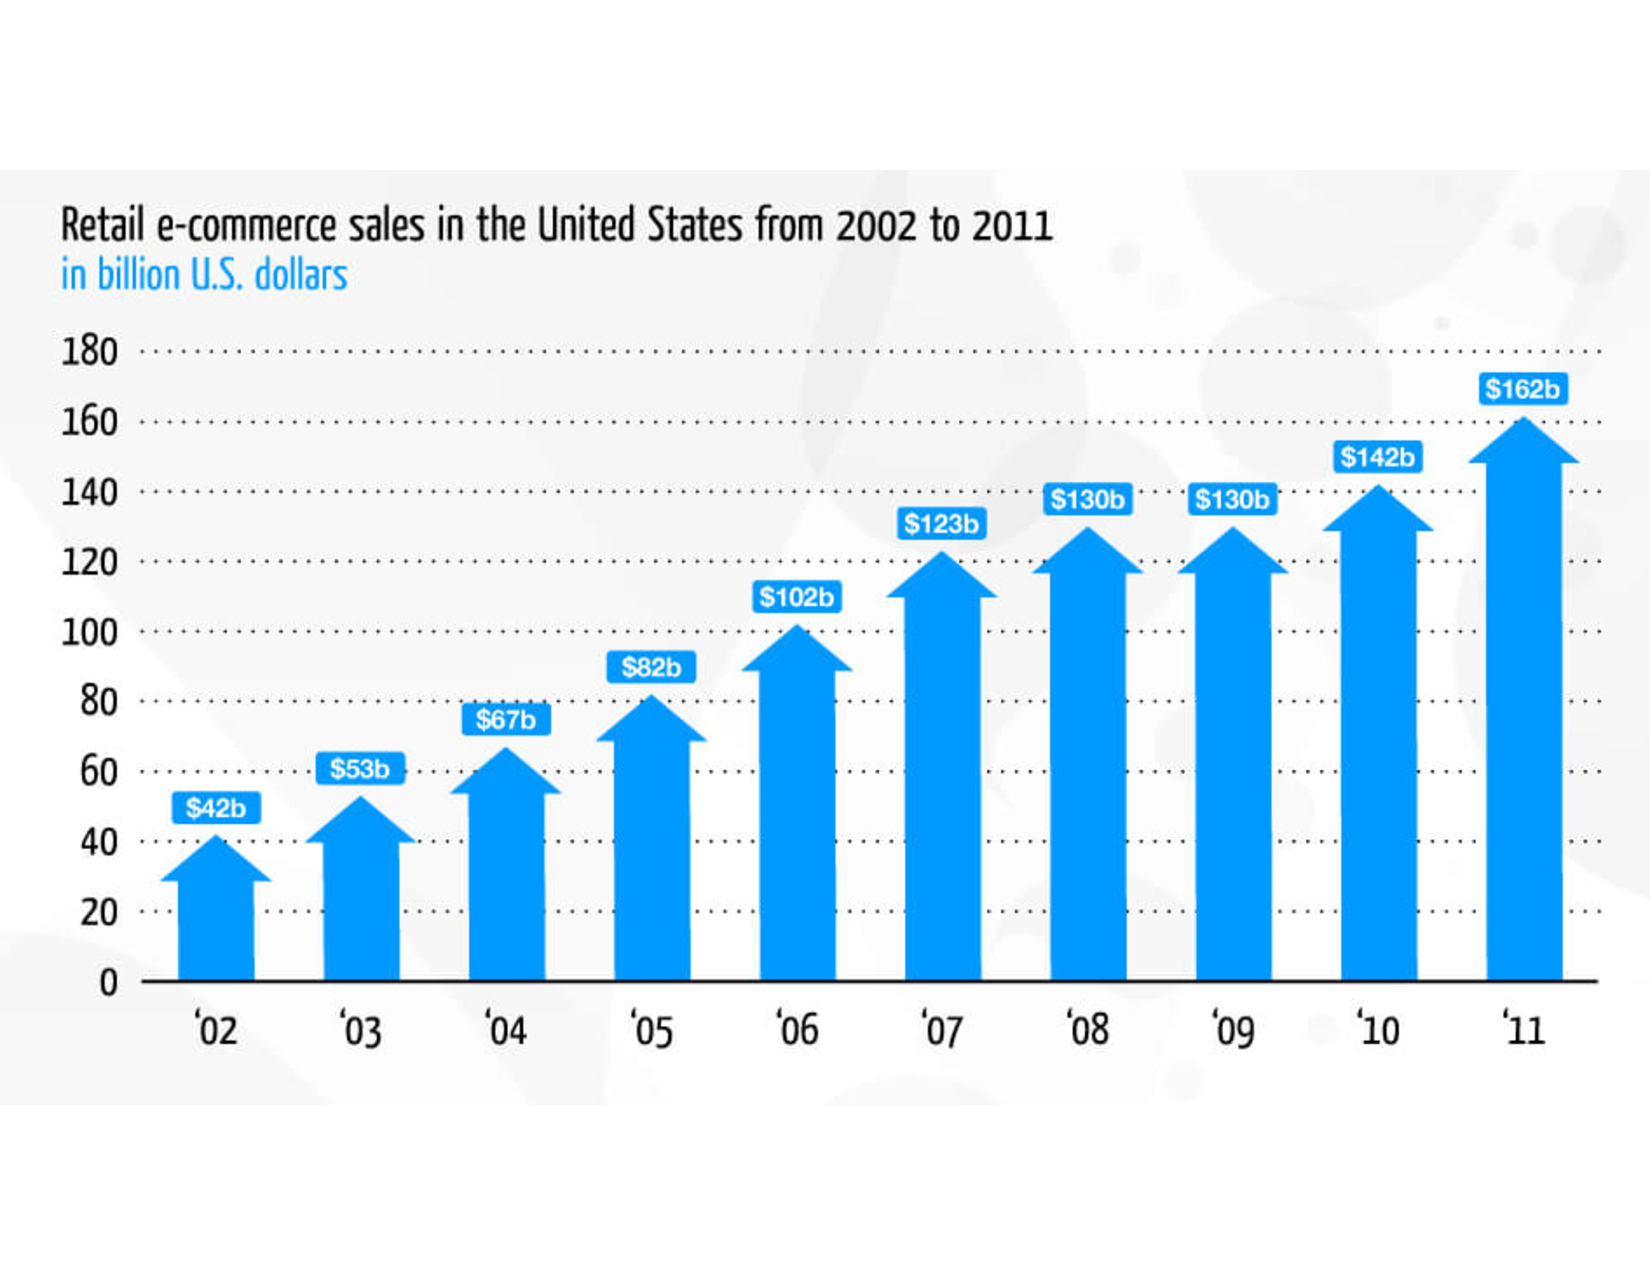
\includegraphics[width=\columnwidth]{eCommerce_chart}}
			\caption{Retail sales in the USA between 2002 and 2011.}
			\label{sales}
		\end{center}
	\vskip -0.2in
\end{figure} 

\begin{figure}[ht]
	\vskip 0.2in
		\begin{center}
			\centerline{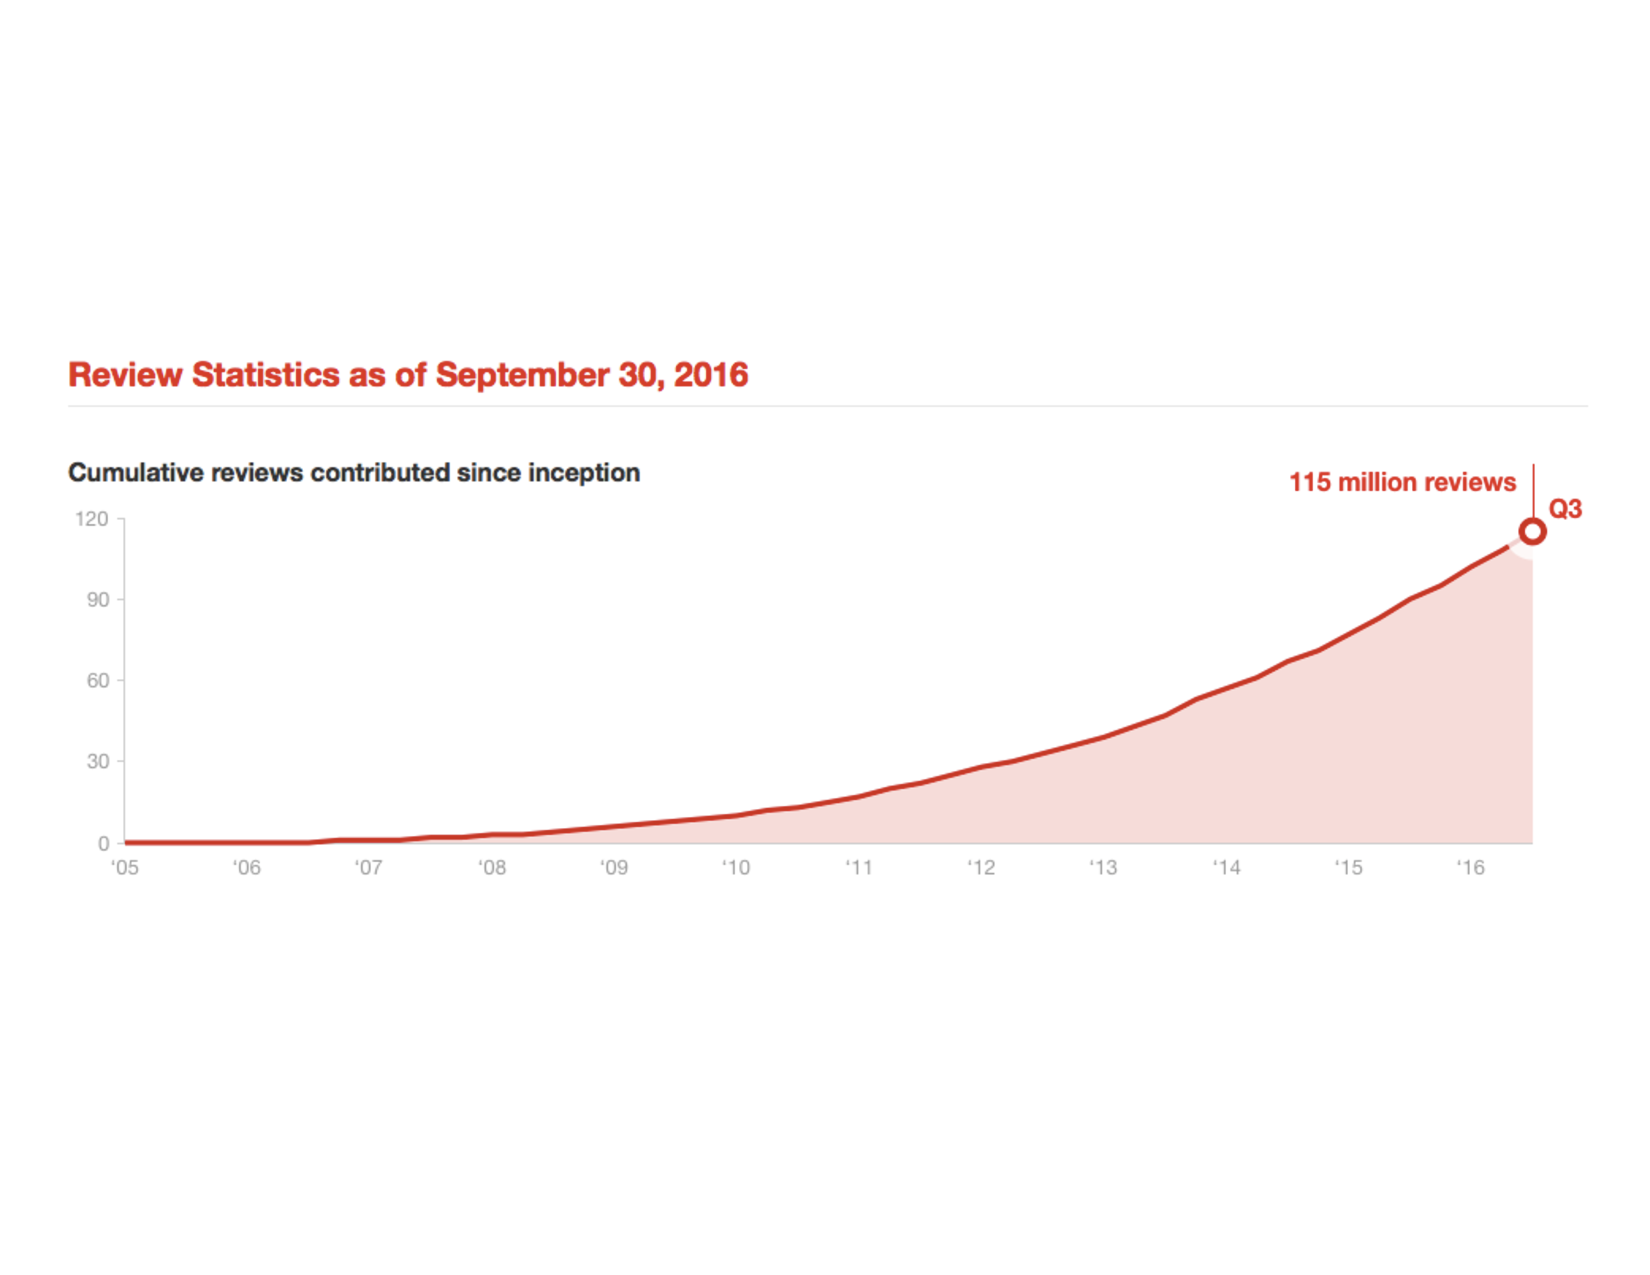
\includegraphics[width=\columnwidth]{yelp_stats}}
			\caption{Yelp Review Statistics}
			\label{yelp}
		\end{center}
	\vskip -0.2in
\end{figure} 


\begin{figure}[ht]
	\centerline{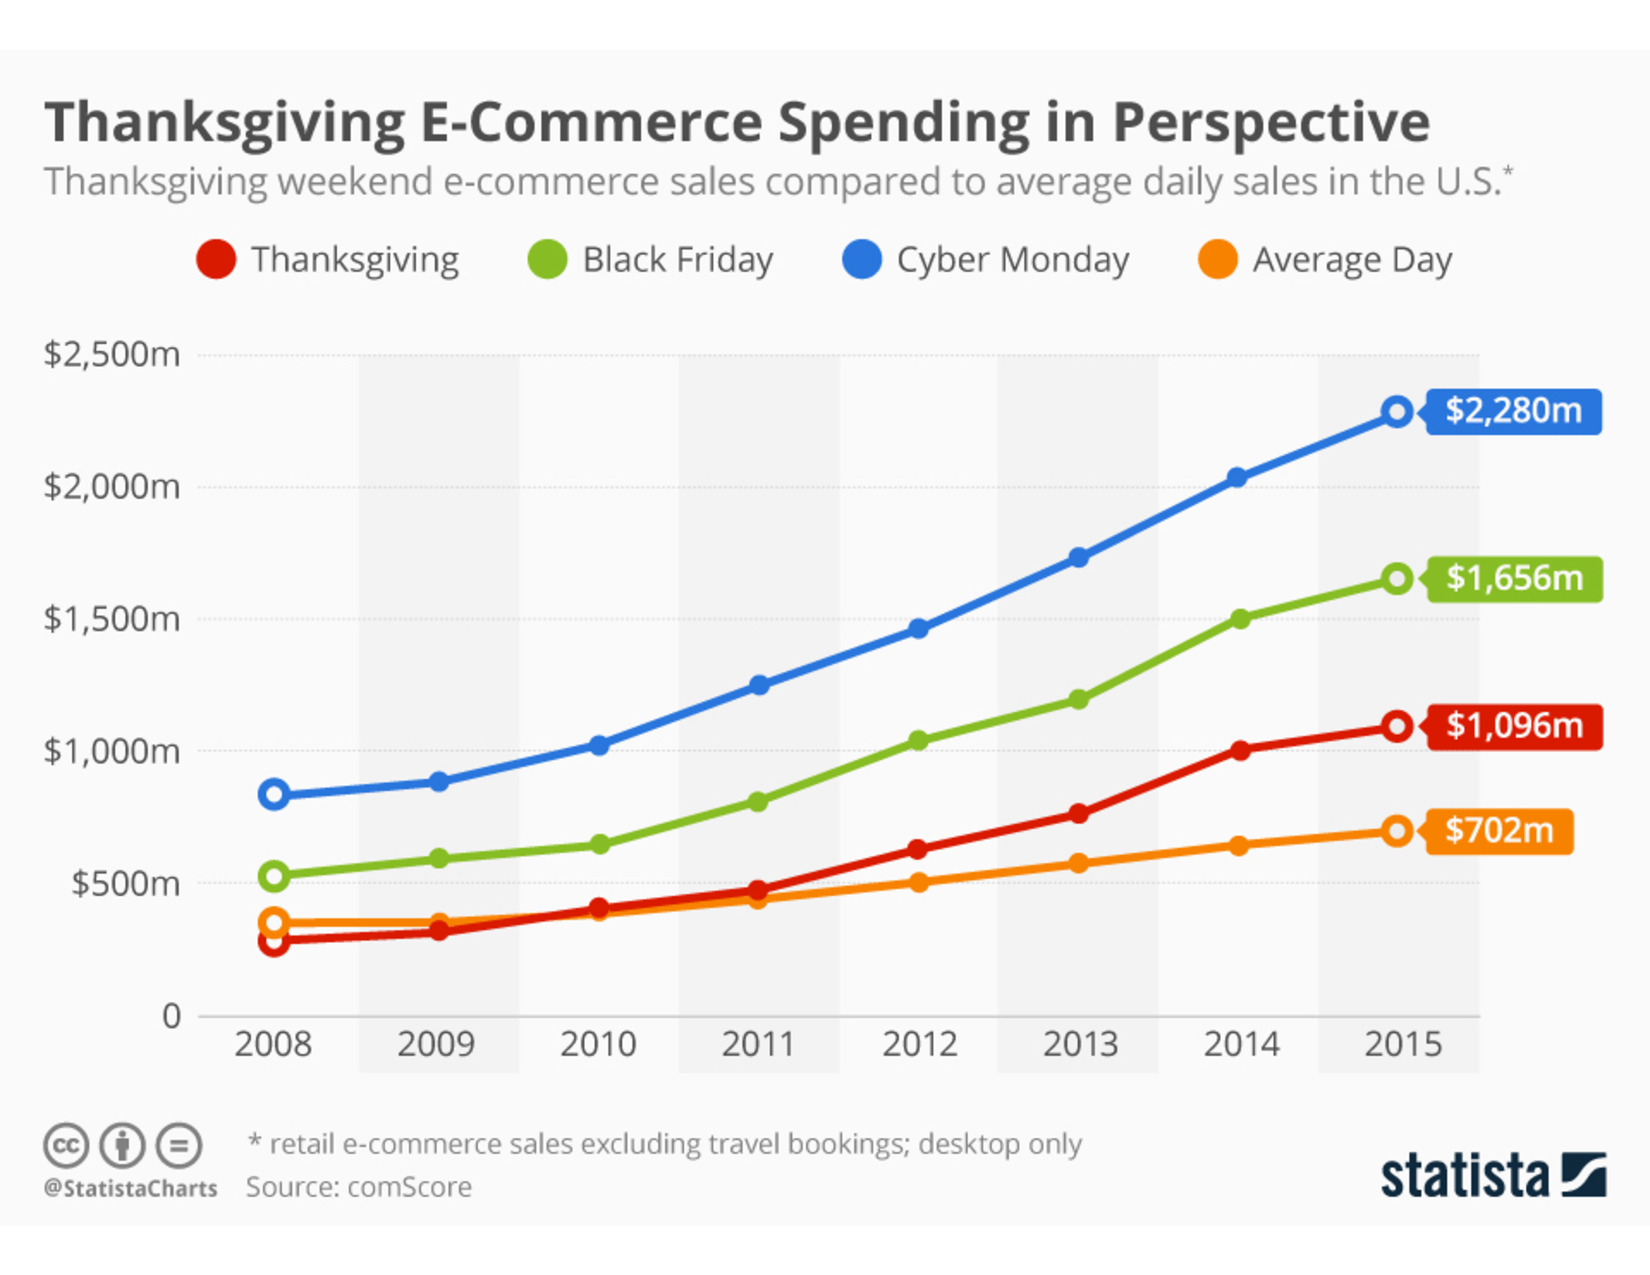
\includegraphics[width=\columnwidth]{Thanksgiving_sales}}
	\caption{eCommerce sales during the Thanksgiving week.}
	\label{thanksgiving}
	\vskip 0.15in
\end{figure} 


\section{Feature Engineering} 
	\label{engineer} 

	

\section{Algorithm Formulation} 
	\label{algorithm} 

	Explain the algorithm...

\section{Evaluation} 
	\label{eval} 

	Enter the evaluation results and parameters used for the evaluation

\section{Results} 
	\label{result} 

	Enter the results obtained after performing the evaluations... 

\section{Deliverables}
	\label{time}
	
	Enter all that could be done in case more time was available... 
	

\begin{thebibliography}{9}
	\bibitem{latexcompanion} 
	A. A.Yeung. 
\textit{Matrix Factorization: Implementation in Python}. 
2010.
 
\bibitem{griffith} 
	T. L. Griffith, M. Steyvers. 
	\textit{Finding Scientific Topics} 	
	PNAS, vol. 10, 6 April - 2004.
 
\bibitem{zhai} 
	Ke Zhai, Jordan Boyd-Graber. 
	\textit{Online Latent Dirichlet Allocation with Infinite Vocabulary} 
	In proceedings, \textit{0th International Conference on Machine Learning}, Atlanta,GA, 2013
	JMLR : W&CP volume 28. Copyright 2013 by the author

\bibitem{lda} 
	D .M. Blei, A. Y. Ng, M. I. Jordan. 
	\textit{Latent Dirichlet Allocation} 
	Journal of Machine Learning Research. 
	January, 2003

\bibitem{crest} 
	Blei, D. M., Griffiths, T. L., Jordan, M. I., & Tenenbaum, J. B. 
	\textit{Hierarchical topic models and the nested Chinese restaurant process} 
	In Advances in Neural Information Processing Systems 16. Cambridge, MA, USA: MIT Press.
	2004

\bibitem{cmu} 
	Erosheva, E. A. 
	\textit{Grade of membership and latent structure models with applications to disability survey data. } 
	Unpublished doctoral dissertation, Department of Statistics, Carnegie Mellon University.

\bibitem{hoffman} 
	Hofmann, T. 
	\textit{Probabilistic Latent Semantic Analysis.} 
	In Proceedings of the Fifteenth Conference on
	Uncertainty in Artificial Intelligence.

\bibitem{zhuang} 
	Zhuang.L, Jing.F, Zhu.X. 
	\textit{Movie Review Mining and Summarization.} 
	CIKM?06, Arlington, VA, USA, 2006.

\bibitem{hum} 
	Hu.M, Liu.B
	\textit{Mining and Summarizing Customer Reviews.} 
	KDD?04, Seattle, WA, USA. 2004

\bibitem{mcauley} 
	McAuley.J, Leskovec.J
	\textit{Hidden Factors and Hidden Topics: Understanding Rating Dimensions with Review Text} 
	In Proceedings of the 7th ACM conference on Recommender systems, Hong Kong, China. 2013

\end{document} 